\section{On-demand Provisioning for Simulation Workflows}
\label{previous:ondemand}

\citeauthor*{provisioning:ondemand} identify requirements that need to be addressed to make the current approach used for scientific workflows more suitable for scientific simulation work~\autocite{provisioning:ondemand}.
The current approach used in the SimTech SWfMS is based on the assumption of service-oriented computing that services are always running.
This can make sense for business applications with a large, steady stream of transactions.
Scientific workflows however are executed infrequently, but when they are executed they need a lot of resources.
Keeping all those resources running all the time is not efficient, so a more flexible way to allocate and use those resources is needed.
The following requirements where identified to be able to improve this situation: Dynamic allocation as well as release of computing resources, on-demand provisioning and deprovisioning of workflow middleware and infrastructure, and dynamic deployment and undeployment of simulation services and their software stacks.
To fulfill these requirements, they propose a new service binding strategy that supports dynamic service deployment, an approach for dynamic provisioning and deprovisioning of workflow middleware, an architecture that is capable of these dynamic deployment and provisioning operations, and, as part of this architecture, the bootware - the subject of this diploma thesis - that kicks of these dynamic processes~\autocite{provisioning:ondemand}.

\begin{figure}[!htbp]
	\centering
	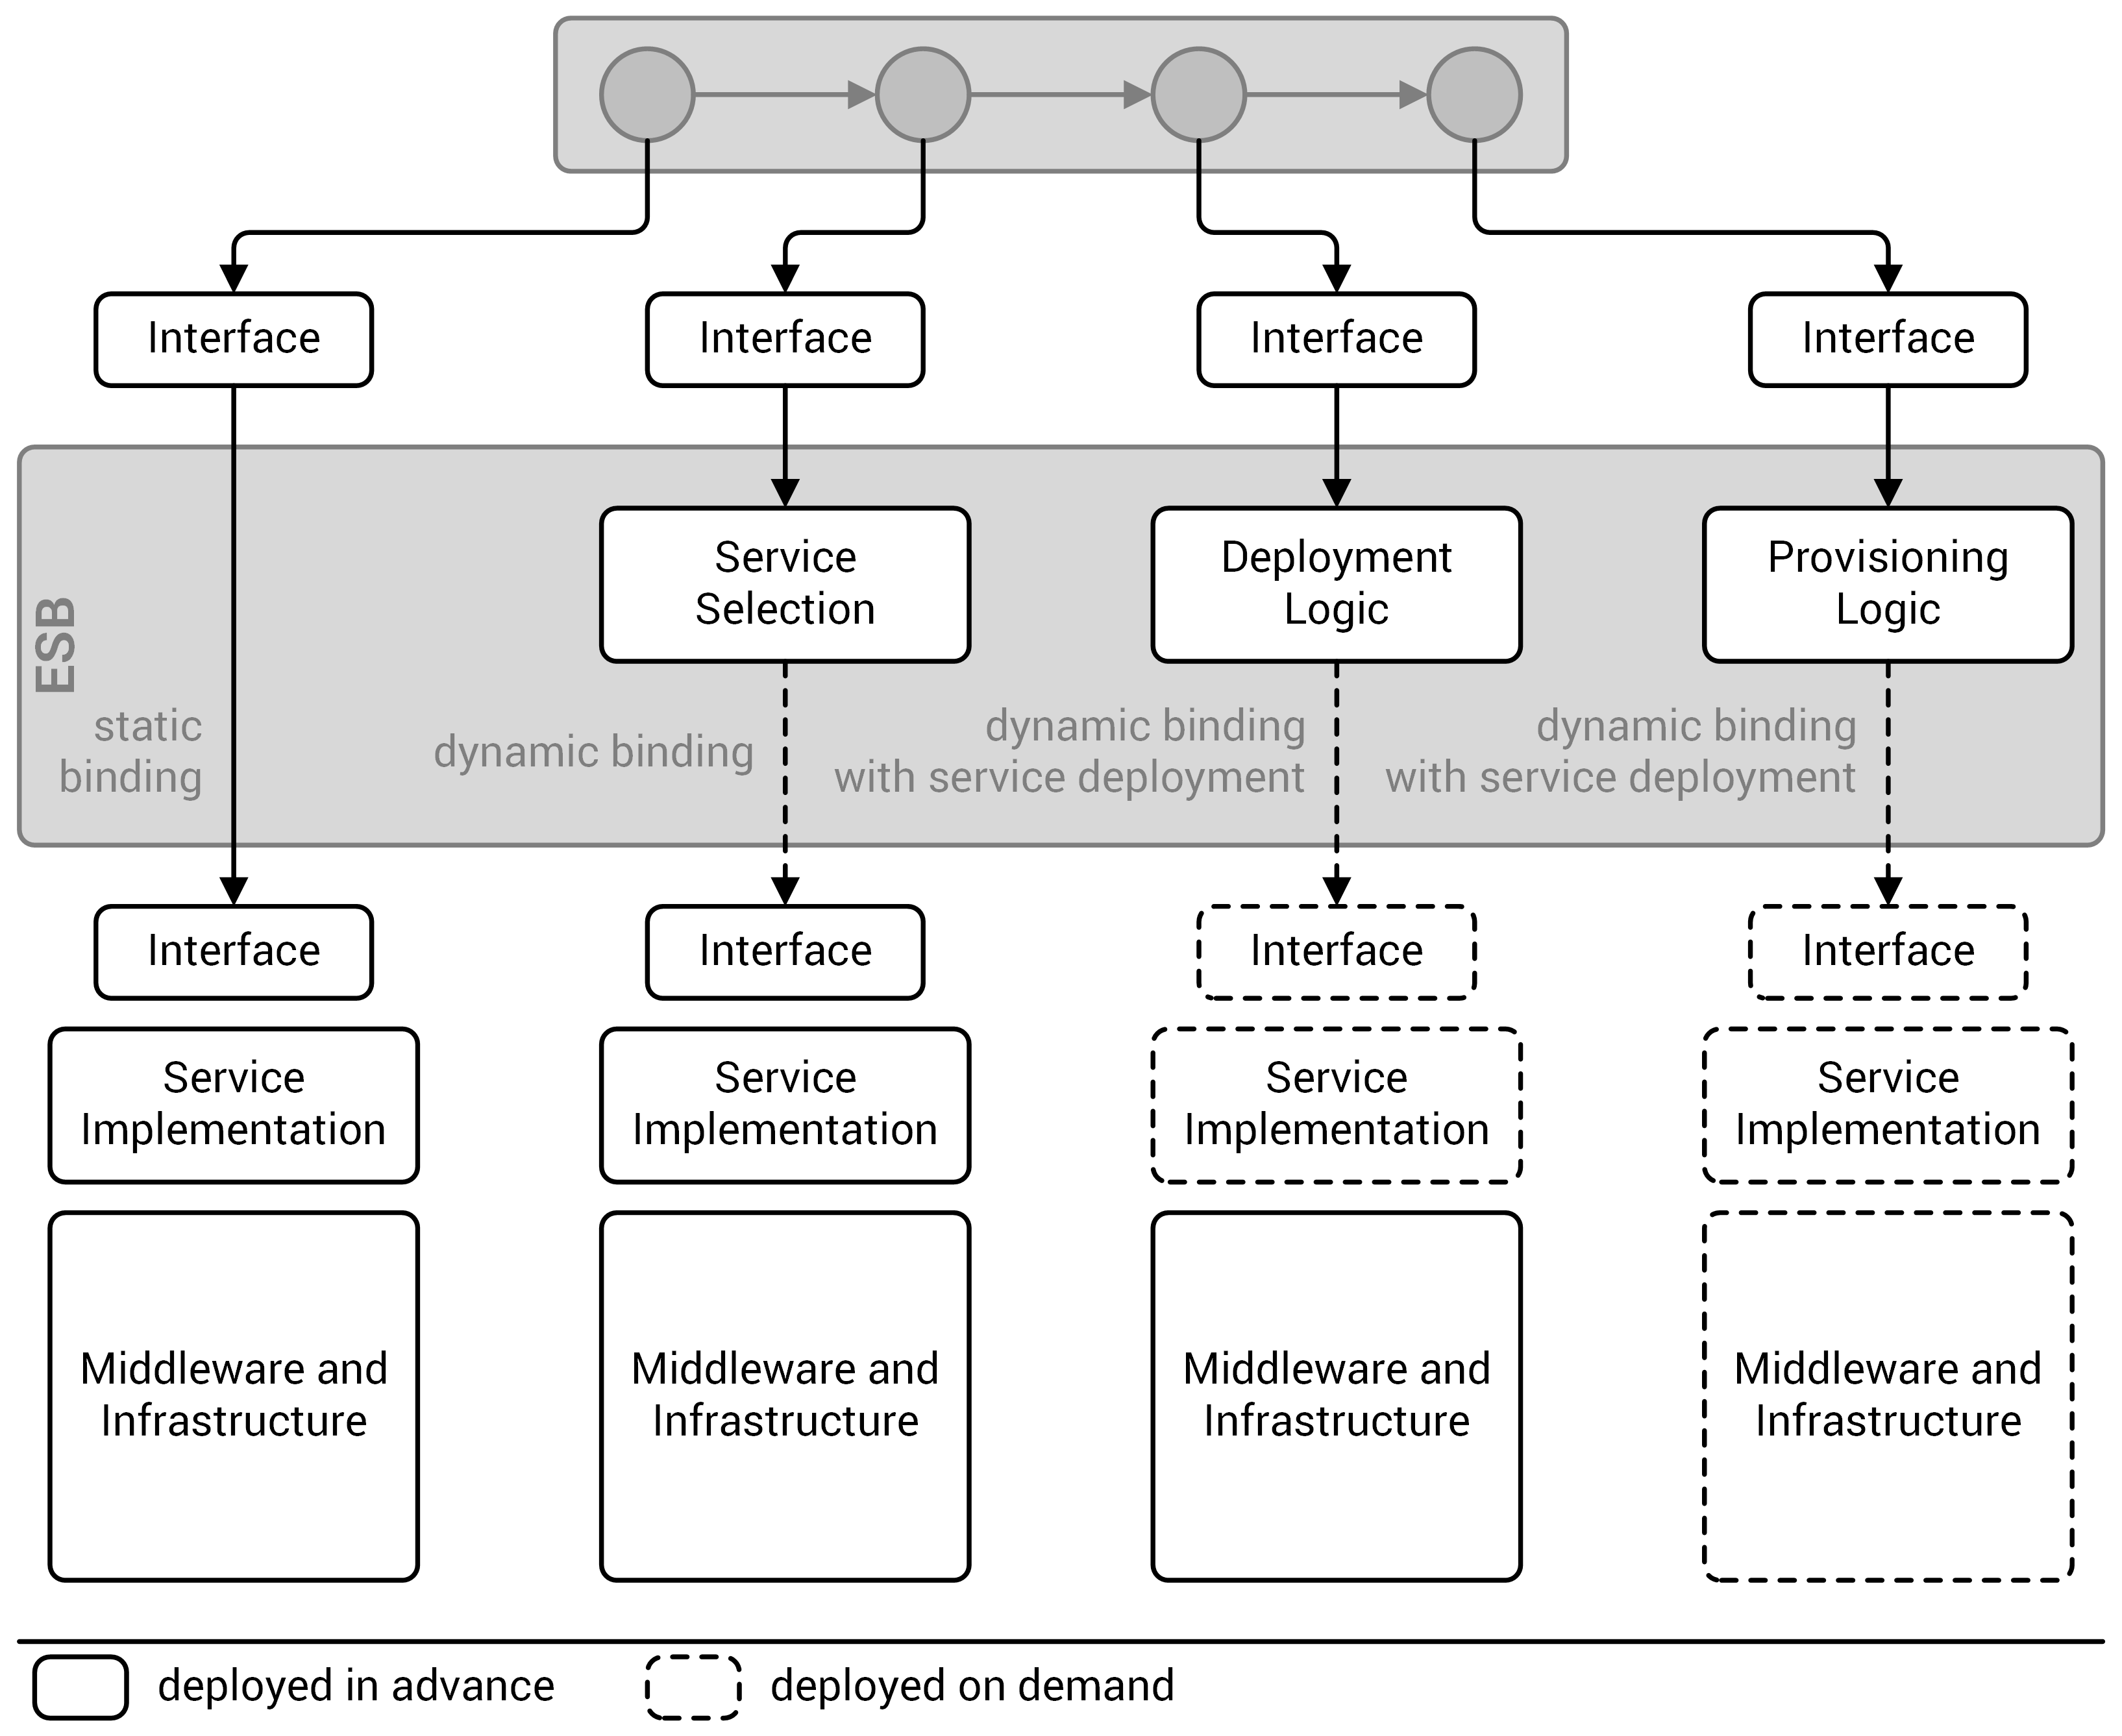
\includegraphics[resolution=600]{previous/assets/service_binding_strategies}
	\caption{Simplified overview of service binding strategies~\autocite[based on][]{provisioning:ondemand}.}
	\label{image:service_binding_strategies}
\end{figure}

The new service binding strategy is necessary, because existing static and dynamic binding strategies, as shown on the left and in the center of \autoref{image:service_binding_strategies}, rely on services that are always running, or, as in the case of dynamic binding with service deployment, only dynamically deploy the service, but not its middleware and infrastructure.
The new service binding strategy, shown on the right of \autoref{image:service_binding_strategies}, called \textit{dynamic binding with software stack provisioning}, is similar to the already existing dynamic binding with service deployment strategy, but adds the dynamic provisioning of the middleware and infrastructure required by the service~\autocite{provisioning:ondemand}.

\begin{figure}[!htbp]
	\centering
	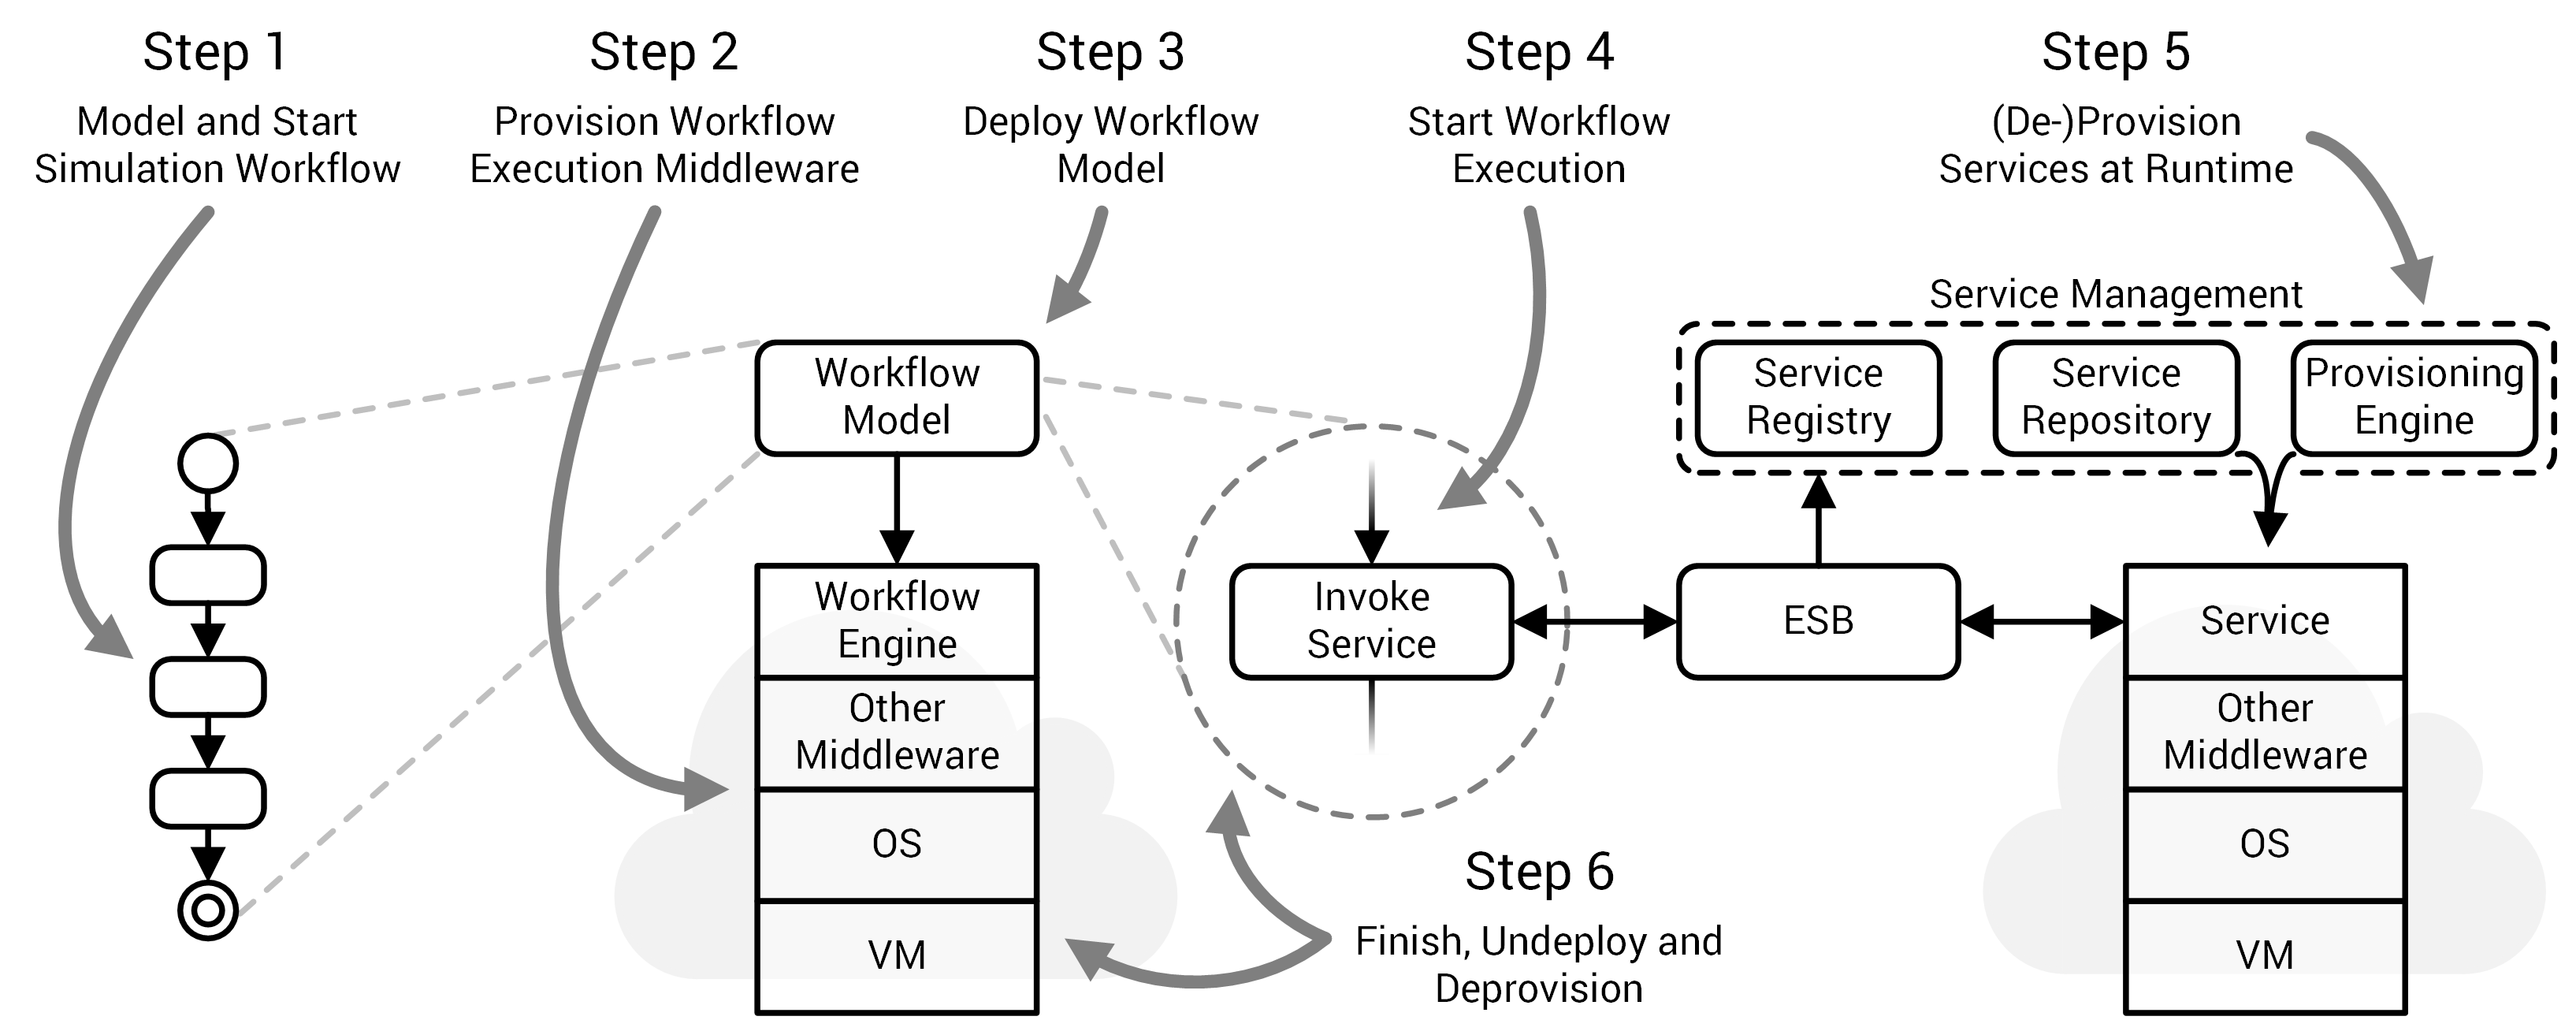
\includegraphics[resolution=600]{previous/assets/provisioning_steps}
	\caption{Steps during the on-demand provisioning of workflow execution middleware and simulation services~\autocite[based on][]{provisioning:ondemand}.}
	\label{image:provisioning_steps}
\end{figure}

Their approach for dynamic provisioning and deprovisioning of workflow middleware and simulation services is separated into six steps, as can be seen in \autoref{image:provisioning_steps}.
The first step is to model and start the execution of a simulation workflow using a local modeling tool like the SimTech Modeler.
In the second step, the middleware for executing the workflow, e.g. the SimTech SWfMS, and its underlying infrastructure are provisioned to a cloud environment.
Now, the workflow can be deployed on this middleware, which is step three.
In step four, an instance of this workflow is executed.
During this execution, a task might invoke some external service that is not yet available.
The ESB determines this by checking the service registry, which stores information about available services.
If the requested service isn't available, the ESB tells the provisioning engine to provision this service.
The on-demand provisioning of services is step five, during which the provisioning engine retrieves the artifacts needed to provision the requested service from the service repository.
The ESB then routes service calls and responses between the invoking workflow activity and the service.
The service is also deprovisioned by the provisioning engine if it is no longer needed.
The final step is to deprovision the workflow model and the workflow execution middleware after the execution of the workflow instance is finished~\autocite{provisioning:ondemand}.

\begin{figure}[!htbp]
	\centering
	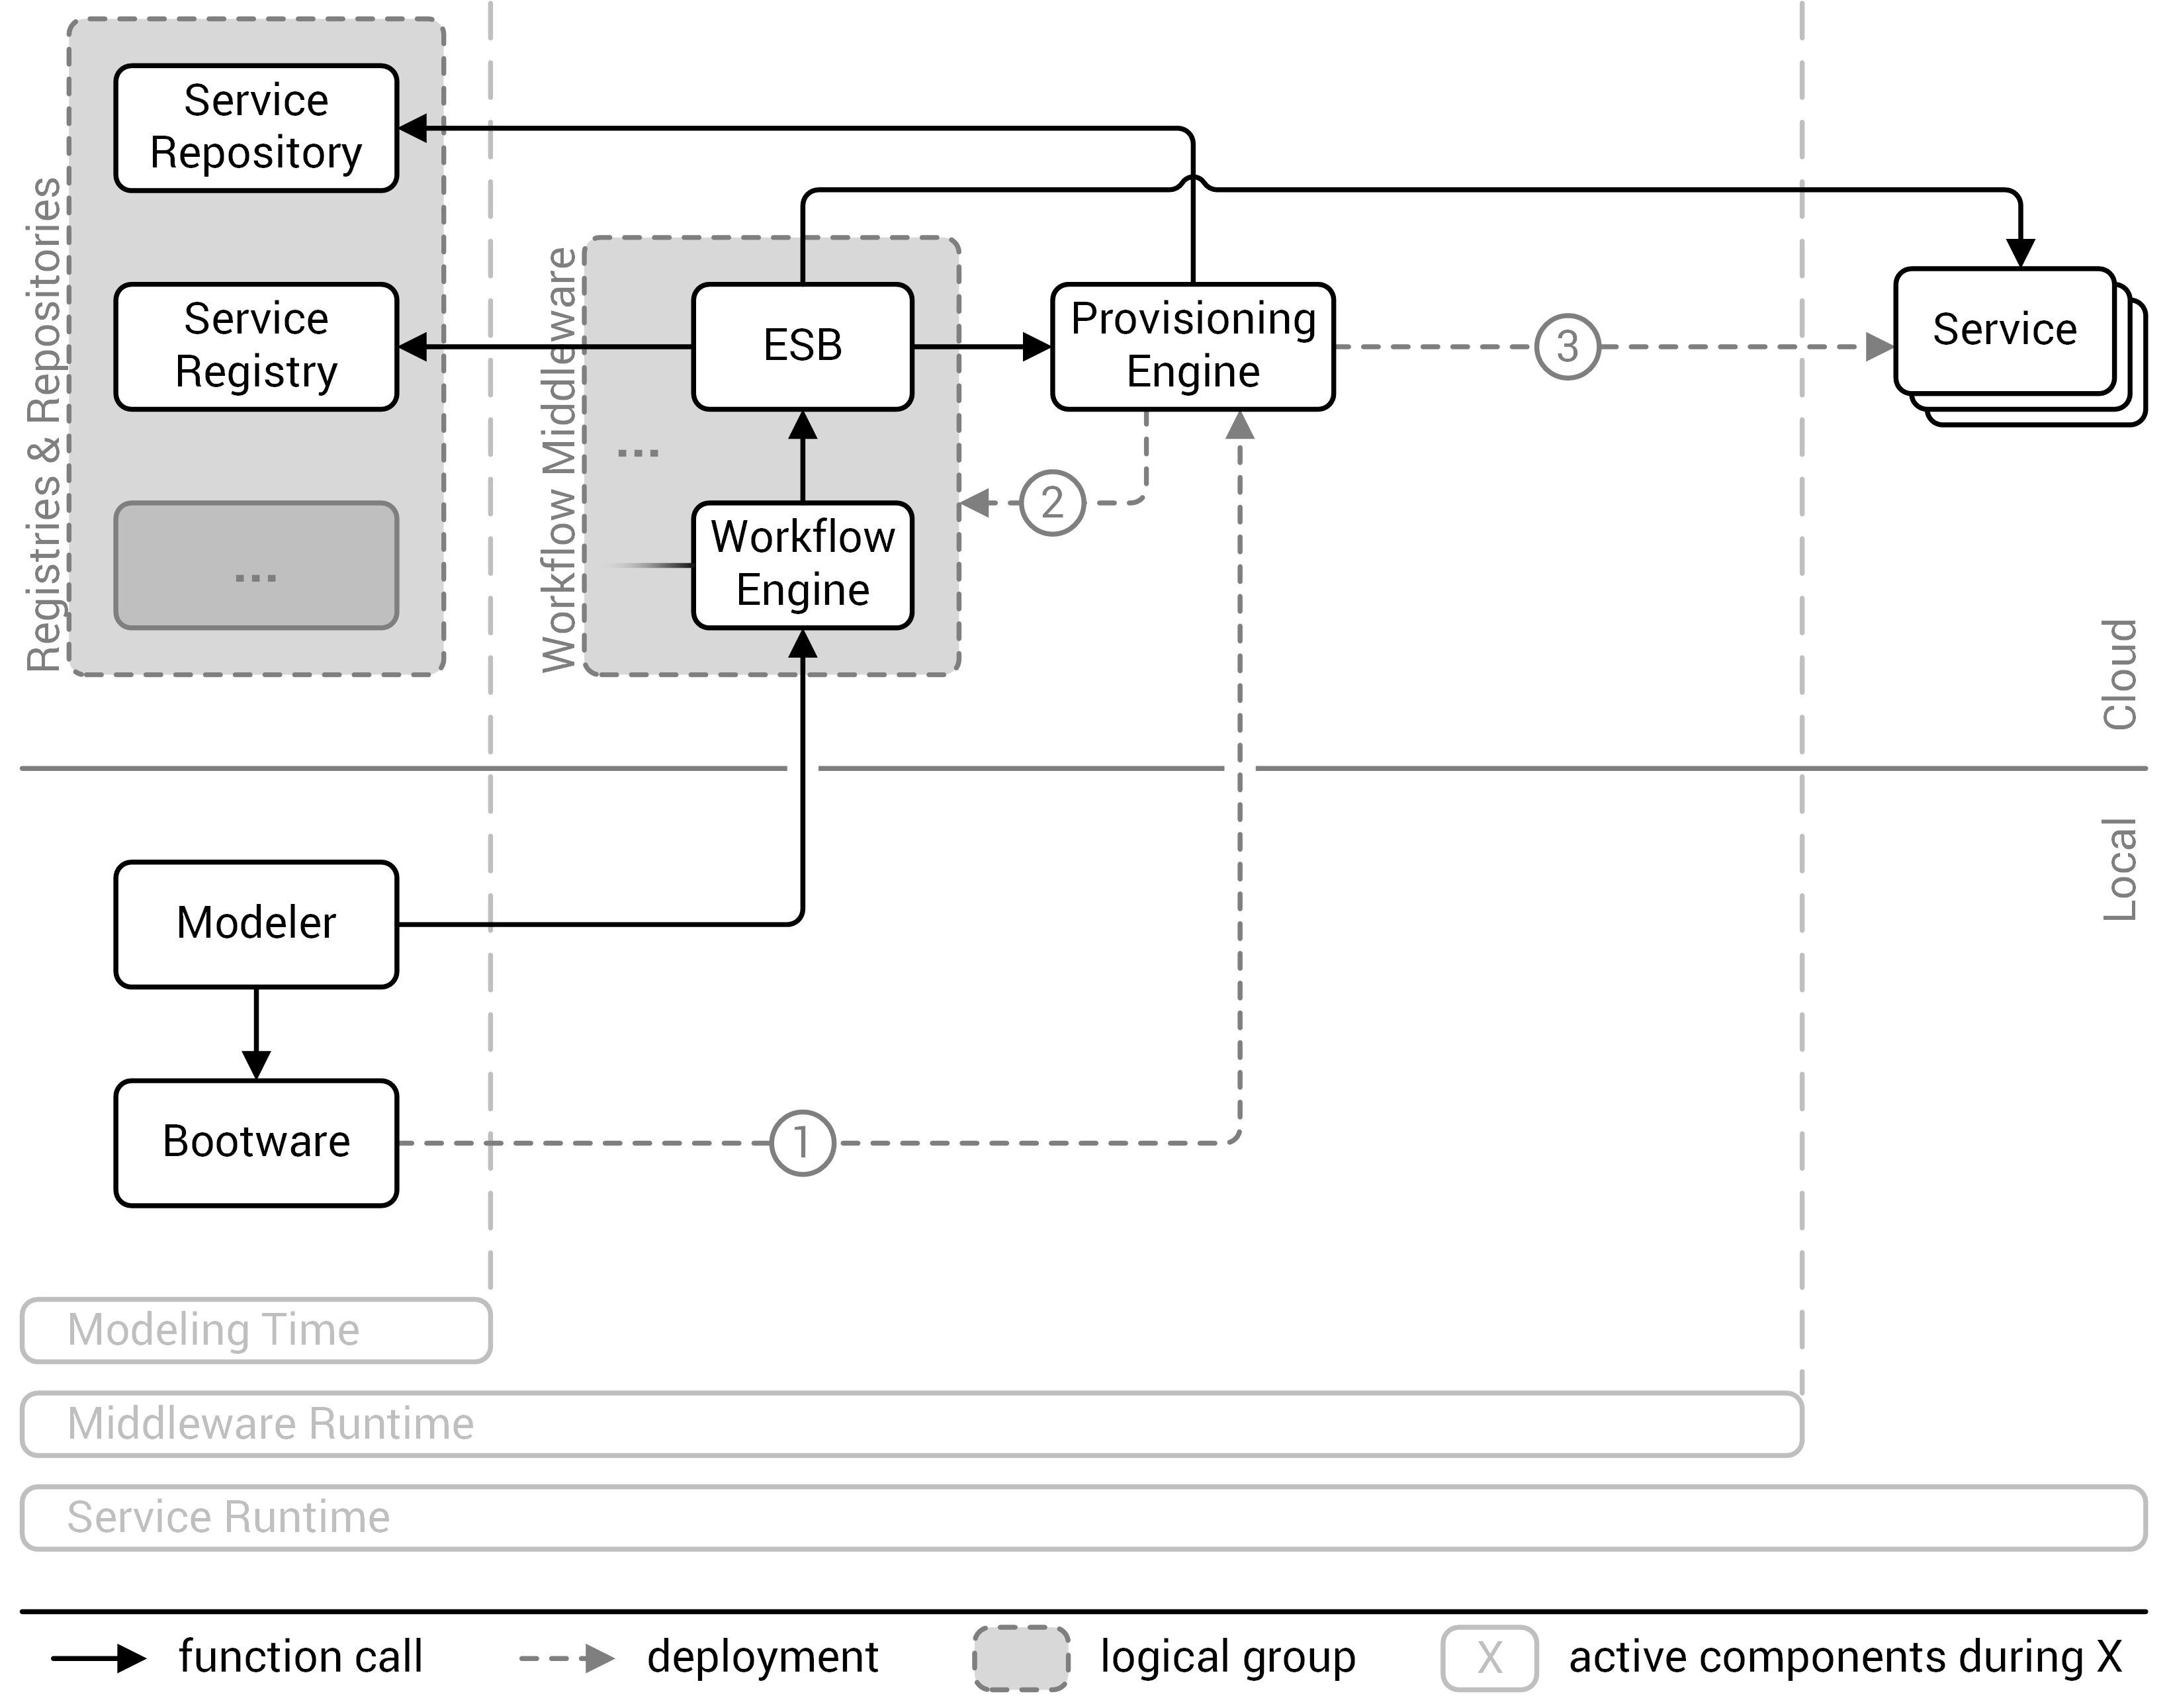
\includegraphics[resolution=600]{previous/assets/original_architecture}
	\caption{Proposed architecture~\autocite[based on][]{provisioning:ondemand}.}
	\label{image:original_architecture}
\end{figure}

The architecture they present, shown in \autoref{image:original_architecture}, can be separated into a local part at bottom and a cloud part at the top, as well as different phases.
The bars at the bottom of \autoref{image:original_architecture} show, which components are active during which phase~\autocite{provisioning:ondemand}.
\autoref{image:original_architecture} shows that the only local components are the modeler and the bootware, while all other components are hosted in the cloud.
In the modeling phase, a scientist uses local modeling and monitoring tools in combination with cloud hosted repositories and registries to create a workflow.
These components are always running.
When he starts the execution of the the workflow, the local bootware component kicks of the on demand provisioning process and therefore the second phase, called middleware runtime phase.
In this phase, the bootware deploys a provisioning engine in the cloud, which in turn deploys the workflow middleware.
Once the middleware is up and running, the workflow can be executed. During the execution, the ESB receives service calls from the workflow engine.
Services that are not running at this time can then be provisioned by the provisioning engine.
This takes place in the third phase, the service runtime phase.

